% !TEX program = pdflatex

\documentclass[a4paper,11pt,twoside]{report}
% THIS FILE SHOULD BE COMPILED BY pdfLaTeX

% ----------------------   PREAMBLE PART ------------------------------

% ------------------------ ENCODING & LANGUAGES ----------------------

\usepackage[utf8]{inputenc}
%\usepackage[MeX]{polski} % Not needed unless You have a name with polish symbols or sth
\usepackage[T1]{fontenc}
\usepackage[english, polish]{babel}


\usepackage{amsmath, amsfonts, amsthm, latexsym} % MOSTLY MATHEMATICAL SYMBOLS

\usepackage[final]{pdfpages} % INPUTING TITLE PDF PAGE - GENERATE IT FIRST!
%\usepackage[backend=bibtex, style=verbose-trad2]{biblatex}


\usepackage{commath} % various commands which can make writing math expressions easier --- documentation available at: https://ctan.gust.org.pl/tex-archive/macros/latex/contrib/commath/commath.pdf

\usepackage[hidelinks]{hyperref} % for hyperlinks, for example, urls, references to equations, entries in a bibliography --- hidelinks option removes rectangles around hiperlinks


% ---------------- MARGINS, INDENTATION, LINESPREAD ------------------

\usepackage[inner=20mm, outer=20mm, bindingoffset=10mm, top=25mm, bottom=25mm]{geometry} % MARGINS


\linespread{1.5}
\allowdisplaybreaks         % ALLOWS BREAKING PAGE IN MATH MODE

\usepackage{indentfirst}    % IT MAKES THE FIRST PARAGRAPH INDENTED; NOT NEEDED
\setlength{\parindent}{5mm} % WIDTH OF AN INDENTATION


%---------------- RUNNING HEAD - CHAPTER NAMES, PAGE NUMBERS ETC. -------------------

\usepackage{fancyhdr}
\pagestyle{fancy}
\fancyhf{}
% PAGINATION: LEFT ALIGNMENT ON EVEN PAGES, RIGHT ALIGNMENT ON ODD PAGES 
\fancyfoot[LE,RO]{\thepage} 
% RIGHT HEADER: zawartość \rightmark do lewego, wewnętrznego (marginesu) 
\fancyhead[LO]{\sc \nouppercase{\rightmark}}
% lewa pagina: zawartość \leftmark do prawego, wewnętrznego (marginesu) 
\fancyhead[RE]{\sc \leftmark}

\renewcommand{\chaptermark}[1]{\markboth{\thechapter.\ #1}{}}

% HEAD RULE - IT'S A LINE WHICH SEPARATES HEADER AND FOOTER FROM CONTENT
\renewcommand{\headrulewidth}{0 pt} % 0 MEANS NO RULE, 0.5 MEANS FINE RULE, THE BIGGER VALUE THE THICKER RULE


\fancypagestyle{plain}{
  \fancyhf{}
  \fancyfoot[LE,RO]{\thepage}
  
  \renewcommand{\headrulewidth}{0pt}
  \renewcommand{\footrulewidth}{0.0pt}
}

% SWOT 
\usepackage{xcolor}
\definecolor{swotS}{RGB}{226,237,143}
\definecolor{swotW}{RGB}{247,193,139}
\definecolor{swotO}{RGB}{173,208,187}
\definecolor{swotT}{RGB}{192,165,184}
\usepackage[raster]{tcolorbox}



% --------------------------- CHAPTER HEADERS ---------------------

\usepackage{titlesec}
\titleformat{\chapter}
  {\normalfont\Large \bfseries}
  {\thechapter.}{1ex}{\Large}

\titleformat{\section}
  {\normalfont\large\bfseries}
  {\thesection.}{1ex}{}
\titlespacing{\section}{0pt}{30pt}{20pt} 

    
\titleformat{\subsection}
  {\normalfont \bfseries}
  {\thesubsection.}{1ex}{}


% ----------------------- TABLE OF CONTENTS SETUP ---------------------------

\def\cleardoublepage{\clearpage\if@twoside
\ifodd\c@page\else\hbox{}\thispagestyle{empty}\newpage
\if@twocolumn\hbox{}\newpage\fi\fi\fi}


% THIS MAKES DOTS IN TOC FOR CHAPTERS
\usepackage{etoolbox}
\makeatletter
\patchcmd{\l@chapter}
  {\hfil}
  {\leaders\hbox{\normalfont$\m@th\mkern \@dotsep mu\hbox{.}\mkern \@dotsep mu$}\hfill}
  {}{}
\makeatother

\usepackage{titletoc}
\makeatletter
\titlecontents{chapter}% <section-type>
  [0pt]% <left>
  {}% <above-code>
  {\bfseries \thecontentslabel.\quad}% <numbered-entry-format>
  {\bfseries}% <numberless-entry-format>
  {\bfseries\leaders\hbox{\normalfont$\m@th\mkern \@dotsep mu\hbox{.}\mkern \@dotsep mu$}\hfill\contentspage}% <filler-page-format>

\titlecontents{section}
  [1em]
  {}
  {\thecontentslabel.\quad}
  {}
  {\leaders\hbox{\normalfont$\m@th\mkern \@dotsep mu\hbox{.}\mkern \@dotsep mu$}\hfill\contentspage}

\titlecontents{subsection}
  [2em]
  {}
  {\thecontentslabel.\quad}
  {}
  {\leaders\hbox{\normalfont$\m@th\mkern \@dotsep mu\hbox{.}\mkern \@dotsep mu$}\hfill\contentspage}
\makeatother



% ---------------------- TABLES AD FIGURES NUMBERING ----------------------

\renewcommand*{\thetable}{\arabic{chapter}.\arabic{table}}
\renewcommand*{\thefigure}{\arabic{chapter}.\arabic{figure}}


% ------------- DEFINING ENVIRONMENTS FOR THEOREMS, DEFINITIONS ETC. ---------------

\makeatletter
\newtheoremstyle{definition}
{3ex}%                           % Space above
{3ex}%                           % Space below
{\upshape}%                      % Body font
{}%                              % Indent amount
{\bfseries}%                     % Theorem head font
{.}%                             % Punctuation after theorem head
{.5em}%                          % Space after theorem head, ' ', or \newline
{\thmname{#1}\thmnumber{ #2}\thmnote{ (#3)}}
\makeatother

\theoremstyle{definition}
\newtheorem{theorem}{Theorem}[chapter]
\newtheorem{lemma}[theorem]{Lemma}
\newtheorem{example}[theorem]{Example}
\newtheorem{proposition}[theorem]{Proposition}
\newtheorem{corollary}[theorem]{Corollary}
\newtheorem{definition}[theorem]{Definition}
\newtheorem{remark}[theorem]{Remark}

% --------------------- END OF PREAMBLE PART (MOSTLY) --------------------------





% -------------------------- USER SETTINGS ---------------------------

\renewcommand{\title}{Platform for hybrid learning}
\newcommand{\type}{Engineer} % Master OR Engineer
\newcommand{\supervisor}{DEng Janusz Oleniacz} % TITLE AND NAME OF THE SUPERVISOR



\begin{document}
\sloppy
\selectlanguage{english}


\includepdf[pages=-]{titlepage} % THIS INPUTS THE TITLE PAGE

\null\thispagestyle{empty}\newpage

% ------------------ PAGE WITH SIGNATURES --------------------------------

%\thispagestyle{empty}\newpage
%\null
%
%\vfill
%
%\begin{center}
%\begin{tabular}[t]{ccc}
%............................................. & \hspace*{100pt} & .............................................\\
%supervisor's signature & \hspace*{100pt} & author's signature
%\end{tabular}
%\end{center}
%


% ---------------------------- ABSTRACTS -----------------------------

{  \fontsize{12}{14} \selectfont
\begin{abstract} 
	\begin{center}
		\title  
	\end{center}
The platform for hybrid learning intends to demonstrate, how the design of educational software could be done using a non-object-oriented approach alongside applying principles of cloud computing.
As students, during the pandemic of 2020-2021, we have seen how the educational system was struggling to handle such a change. Meanwhile, we have also discovered the advantages of studying online - it gave us a great level of flexibility and the possibility to re-access materials (in particular). Keeping in mind, that teachers would also benefit from the re-design of the current approach to knowledge transfer, we decided to try and implement a platform, that covers the interests of both groups. 
We did that using Rust programming language for our backend system, Elm programming language for the frontend, and Azure as a main hosting solution. This paper addresses the obstacles to implementing such a platform and how it differs from already existing solutions. We used our professional knowledge as acting software engineers and students to identify and solve arising issues. 
It is worth adding, that we do not focus on the software development pipeline here, as it would differ vastly from the real-world development team. Nevertheless, we address usability, extendability, supportability, and other important software traits, since they are crucial to the success of the design itself. \\

\noindent \textbf{Keywords:} hydrid learning, massive open online courses, functional programming, cloud computing, education
\end{abstract}
}

\null\thispagestyle{empty}\newpage


% {\selectlanguage{polish} \fontsize{12}{14}\selectfont
% \begin{abstract}

% \begin{center}
% \tytul
% \end{center}

% Lorem ipsum dolor sit amet, consetetur sadipscing elitr, sed diam nonumyeirmod tempor invidunt ut labore et dolore magna aliquyam erat, sed diamvoluptua. At vero eos et accusam et justo duo dolores et ea rebum. Stet clita kasd gubergren, no sea takimata sanctus est Lorem ipsum dolor sit amet.

% Lorem ipsum dolor sit amet, consetetur sadipscing elitr, sed diam nonumyeirmod tempor invidunt ut labore et dolore magna aliquyam erat, sed diamvoluptua. At vero eos et accusam et justo duo dolores et ea rebum. Stet clita kasd gubergren, no sea takimata sanctus est Lorem ipsum dolor sit amet.\\

% \noindent \textbf{Słowa kluczowe:} slowo1, slowo2, ...
% \end{abstract}
% }


%% --------------------------- DECLARATIONS ------------------------------------
%
%%
%%	IT IS NECESSARY OT ATTACH FILLED-OUT AUTORSHIP DEECLRATION. SCAN (IN PDF FORMAT) NEEDS TO BE PLACED IN scans FOLDER AND IT SHOULD BE CALLED, FOR EXAMPLE, DECLARATION_OF_AUTORSHIP.PDF. IF THE FILENAME OR FILEPATH IS DIFFERENT, THE FILEPATH IN THE NEXT COMMAND HAS TO BE ADJUSTED ACCORDINGLY.
%%
%%	command attacging the declarations of autorship
%%
%\includepdf[pages=-]{scans/declaration-of-autorship}
%\null\thispagestyle{empty}\newpage
%
%% optional declaration
%%
%%	command attaching the declaataration on granting a license
%%
%\includepdf[pages=-]{scans/declaration-on-granting-a-license}
%%
%%	.tex corresponding to the above PDF files are present in the 3. declarations folder 
%
\chapter*{History of changes}
\begin{tabular}{ |p{3cm}|p{3cm}|p{7cm}|  }
 	\hline
 	\multicolumn{3}{|c|}{Table of changes} \\
 	\hline
 	Author & Date & Change\\
 	\hline
 	Kiryl Volkau   & 20.10.2021    & add: Abstract, Introduction \\
	Kiryl Volkau   & 20.10.2021    & add: Functional requirements \\
 	Illia Manzhela &  20.10.2021  & add: Non-functional requirements \\
 	Illia Manzhela &  20.10.2021  & add: SWOT analysis, schedule \\
 	\hline
\end{tabular}
% ------------------- TABLE OF CONTENTS ---------------------
% \selectlanguage{english} - for English
\pagenumbering{gobble}
\tableofcontents
\thispagestyle{empty}
\newpage % IF YOU HAVE EVEN QUANTITY OD PAGES OF TOC, THEN REMOVE IT OR ADD \null\newpage FOR DOUBLE BLANK PAGE BEFORE INTRODUCTION


% -------------------- THE BODY OF THE THESIS --------------------------------

\null\thispagestyle{empty}\newpage
\pagestyle{fancy}
\pagenumbering{arabic}
\setcounter{page}{11}

\chapter*{Vocabulary}
\markboth{}{Vocabulary}
\addcontentsline{toc}{chapter}{Vocabulary}


\begin{enumerate}
\item \textbf{Massive Open Online Courses (MOOC)} platform - platform with educational content including videos, text content, discussion forums.
\item \textbf{Application Programming Interface (API)} - set of definitions for building and integrating application software.
\item \textbf{Minimal Viable Product (MVP)} - version of product that has enough functionalities to be used by early customers.
\item \textbf{Infrastracture as a Service (IaaS} - pay-as-you-go service where a third party provides you with infrastructure services, like storage and virtualization, as you need them, via a cloud, through the internet. \href{https://www.redhat.com/en/topics/cloud-computing/iaas-vs-paas-vs-saas}{https://www.redhat.com/en/topics/cloud-computing/iaas-vs-paas-vs-saas}
\item \textbf{Platform as a Service (PaaS}) - on-premise infrastructure management where a provider hosts the hardware and software on its own infrastructure and delivers this platform to the user as an integrated solution, solution stack, or service through an internet connection. \href{https://www.redhat.com/en/topics/cloud-computing/iaas-vs-paas-vs-saas}{https://www.redhat.com/en/topics/cloud-computing/iaas-vs-paas-vs-saas}
\end{enumerate}


\chapter*{Introduction}
\markboth{}{Introduction}
\addcontentsline{toc}{chapter}{Introduction}

What is the thesis about? What is the content of it? What is the Author's contribution to it?
\par
WARNING!  In a diploma thesis which is a team project: Description of the work division in the team, including the scope of each co-author’s contribution to the practical part (Team Programming Project) and the descriptive part of the diploma thesis. 
\par

Lorem ipsum dolor sit amet, consetetur sadipscing elitr, sed diam nonumyeirmod tempor invidunt ut labore et dolore magna aliquyam erat, sed diamvoluptua. At vero eos et accusam et justo duo dolores et ea rebum. Stet clita kasd gubergren, no sea takimata sanctus est Lorem ipsum dolor sit amet. Lorem ipsum dolor sit amet, consetetur sadipscing elitr, sed diam nonumyeirmod tempor invidunt ut labore et dolore magna aliquyam erat, sed diamvoluptua. At vero eos et accusam et justo duo dolores et ea rebum. Stet clita kasd gubergren, no sea takimata sanctus est Lorem ipsum dolor sit amet.

\chapter*{Responsibilities and Schedule}
\markboth{}{Responsibilities and Schedule}
\addcontentsline{toc}{chapter}{Responsibilities and Schedule}
\begin{center}
\begin{tabular}{ |c|c| } 
 \hline
 Full Name & Responsibility \\ 
 \hline
 Kiryl Volkau & Frontend (Elm) \& DevOps (Azure) \\ 
 Illia Manzhella & Backend (Rust) \& DevOps (GitHub Actions) \\ 
 \hline
\end{tabular}
\begin{figure}[h]
    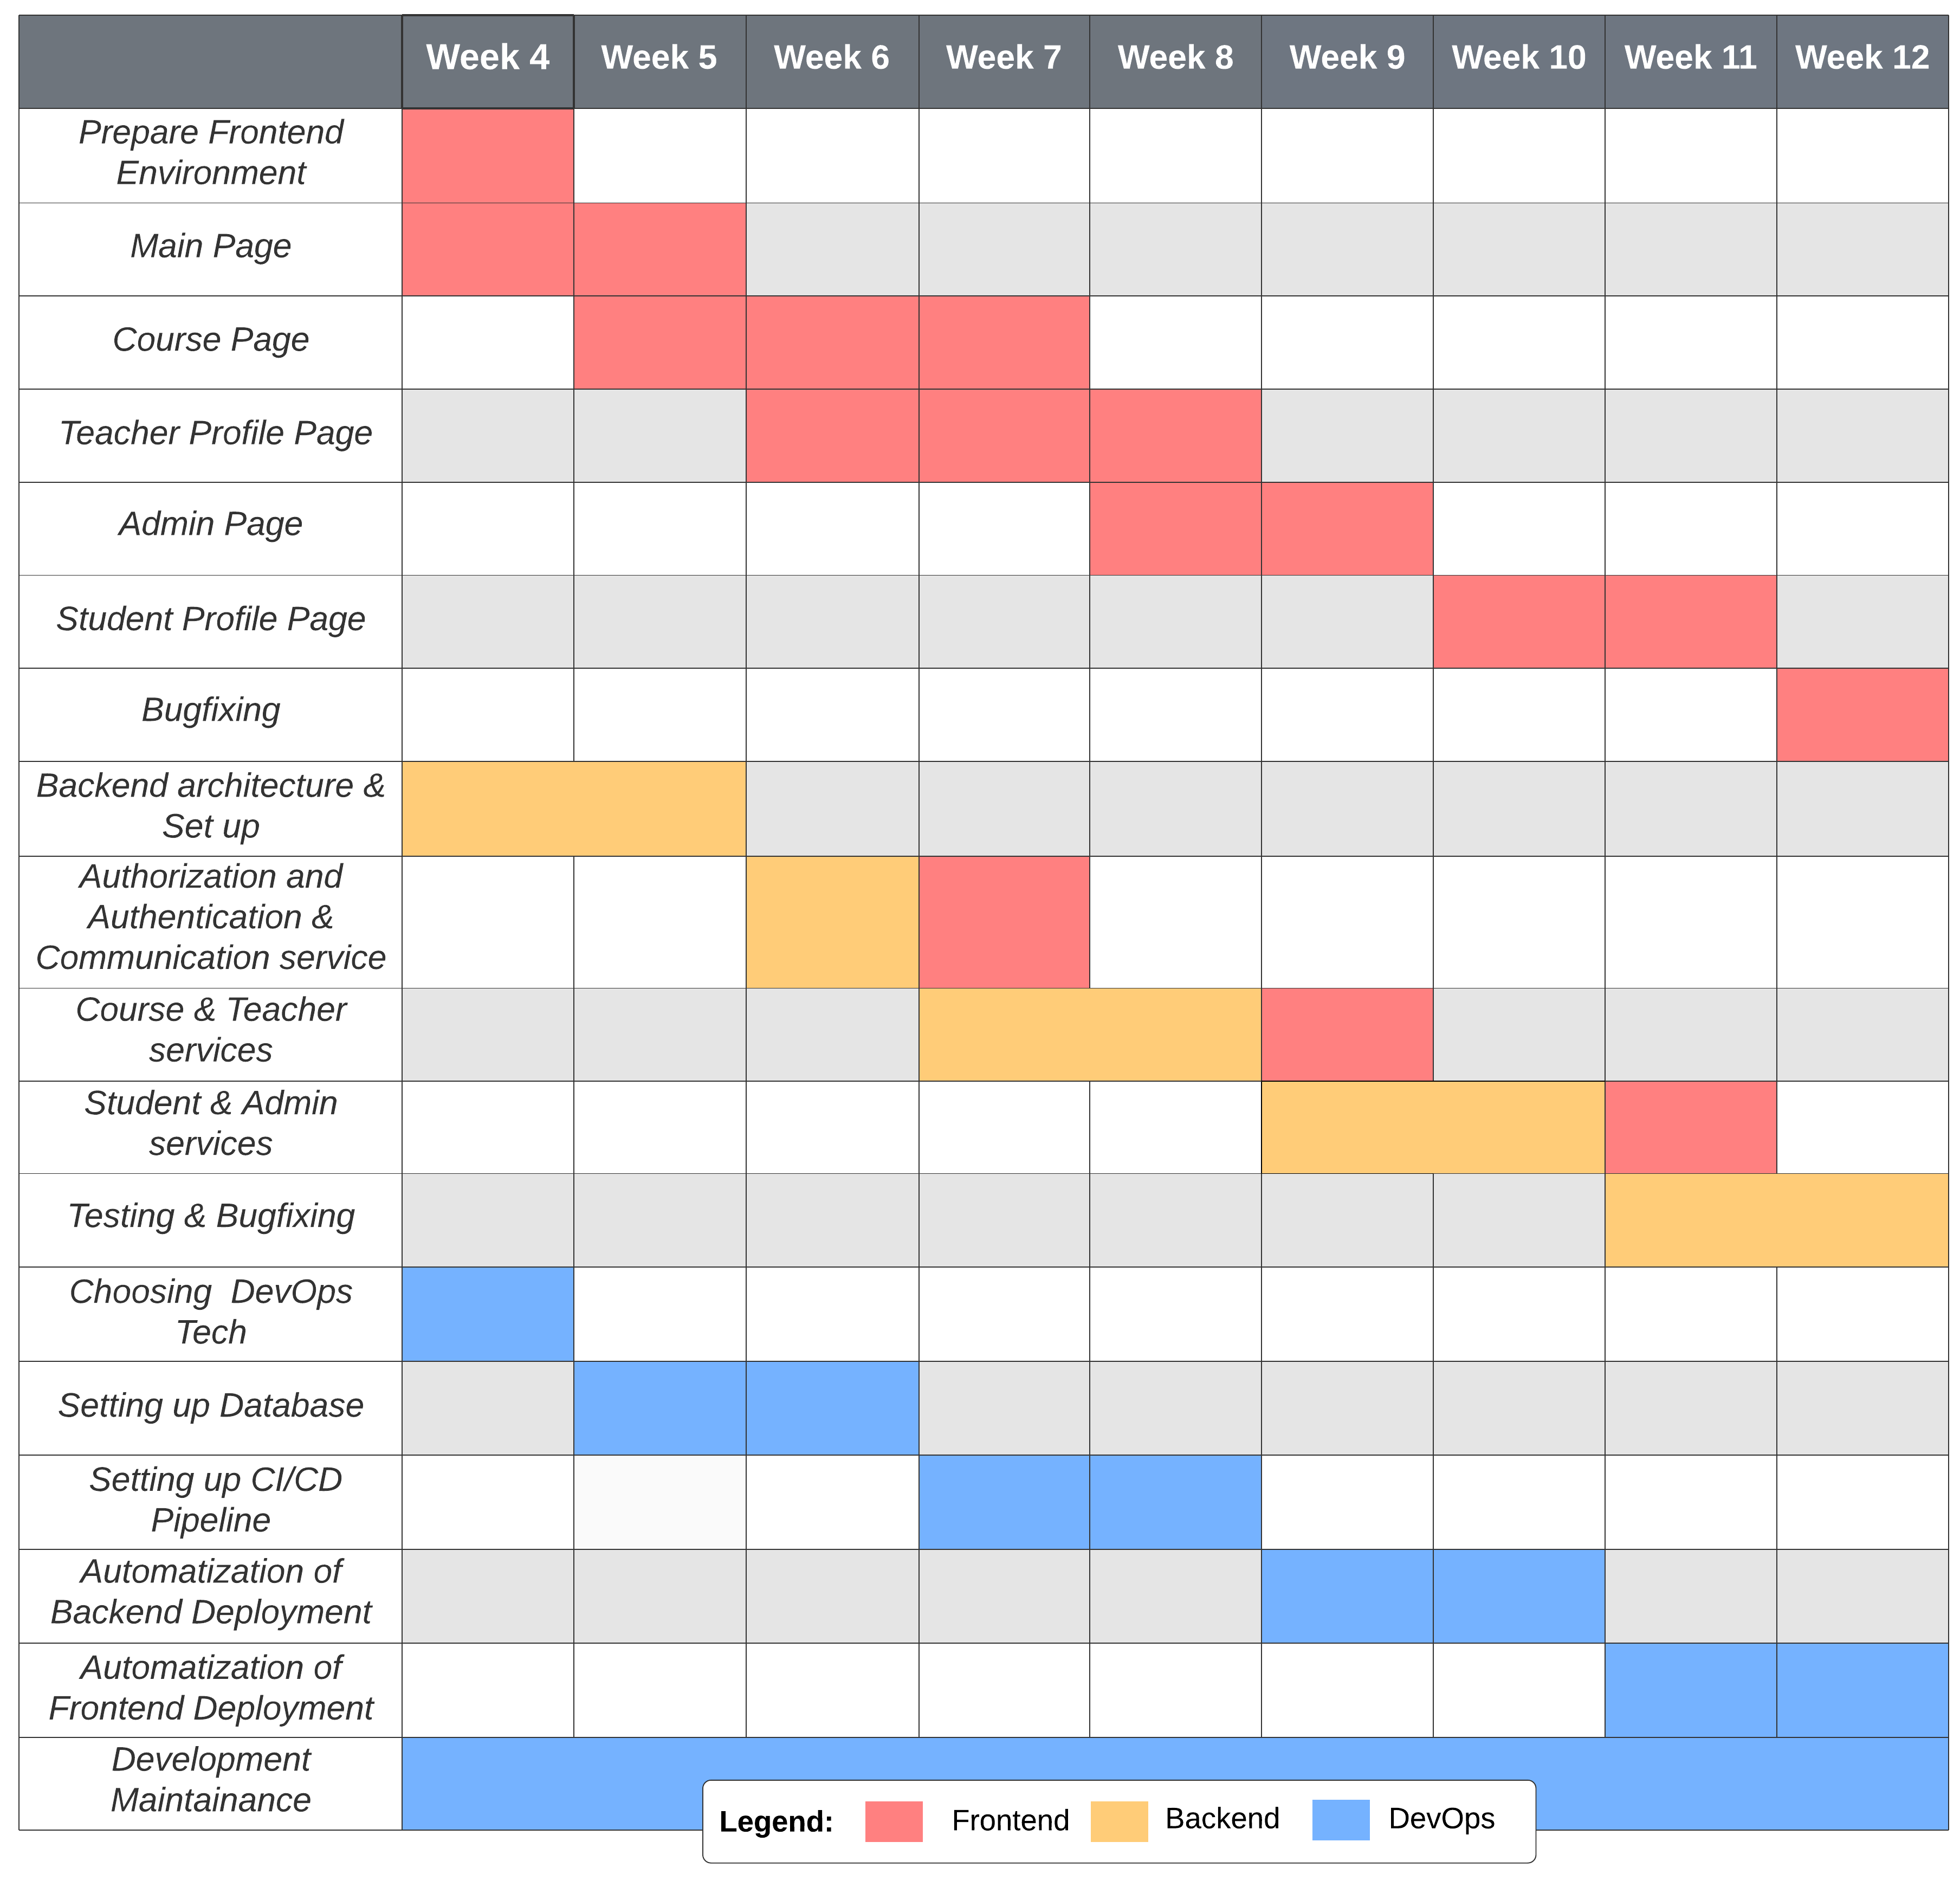
\includegraphics[scale=.52]{img/gantt.png}
    \caption{Gantt chart by task and person}
\end{figure}
\end{center}

\chapter*{Functional Requirements}
\markboth{}{Functional Requirements}
\addcontentsline{toc}{chapter}{Functional Requirements}

We have decided to describe functionality of an application from the users' roles perspective, 
allowing us to represent fuctional requirements as a user stories.
Moreover, it allows us to specify granularity of given access and permissions.

The roles are as follows:
\begin{itemize}
\itemsep0em 
\addtolength{\itemindent}{0.5cm}
	\vspace{-0.2cm}\item Everyone (combines all the groups below)
    \vspace{-0.2cm}\item Anonymous User (Unauthorised)
	\vspace{-0.2cm}\item Everyone Authorised (Teacher, User, Administrator)
    \vspace{-0.2cm}\item Teacher
    \vspace{-0.2cm}\item Student
    \vspace{-0.2cm}\item Administrator
\end{itemize}

\begin{enumerate}
	\itemsep0em 
    \item \textbf{Everyone} can: 
    \begin{itemize}
        \vspace{-0.2cm}\item View universities that has been made public
        \vspace{-0.2cm}\item View university courses (and its contents) that has been made public
        \vspace{-0.2cm}\item Search for courses by name, university, tags
    \end{itemize}
    
    
    \item \textbf{Everyone Authorised} can: 
    \begin{itemize}
        \item Log out
        \item Change personal details
        \item See their University details (if they are hidden from anonymous users)
    \end{itemize}
    
    \item \textbf{Anonymous User} can :
    \begin{itemize}
        \item Create account as student
        \item Create account as teacher
        \item Login to the existing account
    \end{itemize}
    
    \item \textbf{Authenticated User} can :
     \begin{itemize}
        \item See their events calendar
        \item Leave messages on university / courses boards
    \end{itemize}

    \item \textbf{Teacher} can :
     \begin{itemize}
        \item Submit own courses
        \item Change own course information
        \item Delete own course
        \item See students' comments on his/her course
        \item Add additional materials to the course
    \end{itemize}
    
    \item \textbf{University Administrator} can :
    \begin{itemize}
        \item Manage university staff and students
        \item Review submitted university courses
        \item Accept university submitted courses
        \item Reject university submitted courses
        \item Delete university courses (with possibility to recover)
        \item See university students' and teachers' details
        \item Make university courses open
    \end{itemize}

\end{enumerate}

There is also a super-admin role foreseen, which should be used for the 

\chapter*{Non-Functional Requirements}
\markboth{}{Non-Functional Requirements}
\addcontentsline{toc}{chapter}{Non-Functional Requirements}

\begin{enumerate}
\itemsep 0em 
    \item \textbf{Usability} \\
     Level of basic user expertise assumed. User interface standards will be used.
    \item \textbf{Reliability} \\
      Platform will be available 24/7 with the possibility of restarting the system in case of emergency situations (using PaaS / IaaS functionality or kubernetes). Recoverability will be maintained by an engineer who will recover system from a shut-down failure in case of several unsuccessful attempts to restart). It will accessible from the most popular browsers like Google Chrome (and Chromium-based), Safari, Firefox, and Opera.

    \item \textbf{Performance} \\
     System response time is supposed to not exceed 2000ms, automatic recovery and start-up time is expected to take up to 30 minutes. 
     
    \item \textbf{Supportability} \\
     System should be testable, maintainable and easily scalable for the needs of higher throughput of media streaming for large number of students. This includes possibility of refactoring the architecture to be more decoupled. 
     
     \item \textbf{Extendibility} \\ 
     System should be easy to extend - meaning it should be possible to add more features to the existing architecture without significant need for the refactoring of previously implemented system. 
     
\end{enumerate}

\chapter*{SWOT Analysis}
\markboth{}{SWOT Analysis}
\addcontentsline{toc}{chapter}{SWOT Analysis}
\begin{tcbraster}[raster columns=2, boxrule=0mm, arc=0mm]
\begin{tcolorbox}[equal height group=A, size=fbox, colback=swotS!60, colframe=swotS!80!black, title=\textsc{strengths}]
\begin{enumerate}
\item Good understanding of the chosen technologies
\item Team of skilled well-coordinated developers 
\item Milestones are well-defined and understood
\end{enumerate}
\end{tcolorbox}
\begin{tcolorbox}[equal height group=A, size=fbox, colback=swotW!60, colframe=swotW!80!black, title=\textsc{weaknesses}]
\begin{enumerate}
\item Lack of experience with large projects
\item Budget of the project
\item Lack of marketing experience
\end{enumerate}
\end{tcolorbox}
\begin{tcolorbox}[equal height group=B, size=fbox, colback=swotO!60, colframe=swotO!80!black, title=\textsc{opportunities}]
\begin{enumerate}
\item Growing interest in educational products gives more confidence in the success of the product
\item Modernization of the market of educational websites  
\end{enumerate}
\end{tcolorbox}
\begin{tcolorbox}[equal height group=B, size=fbox, colback=swotT!60, colframe=swotT!80!black, title=\textsc{threats}]
\begin{enumerate}
\item Big competition on the market
\item Not enough time to complete the project
\item Absence of team members due to some reasons
\end{enumerate}
\end{tcolorbox}
\end{tcbraster}
\textbf{Threats}
\begin{enumerate}
    \item \textit{Big competition on the market} - as was mentioned in the Introduction, there are already several global players, being Udemy, Udacity, Coursera, etc. Moreover, there are local solutions - like \href{https://navoica.pl}{https://navoica.pl} for Poland offering similar functionality, having well-established processes and budget. Combined with listed above weaknesses - as lack of marketing experience - we may find ourselves in position, when the product is ready, but no one learned about it.
     \item \textit{Not enough time to complete the project} - there is a possibility that such a big project our team will not be able to finish on time. In such scenario, out team is planning to extend the time span for this project for one more semester.
      \item \textit{Absence of team members due to some reasons} - in case of absence of any of the team members for some reason, all the responsibilities of that person will be taken by the other members of the team.
\end{enumerate}


\end{document}
